\documentclass[mathserif,t]{beamer}
%\usepackage{Sweave}                                                       
%http://tex.stackexchange.com/questions/105613/footer-in-beamer. Check this out. Frankfurt template.
%http://tex.stackexchange.com/questions/39345/piecewise-highlighting-in-beamer-presentation
\usepackage{amssymb,bm,mathtools,amsmath}                                                      
\usepackage{graphicx,caption,float}
\usepackage[UKenglish]{isodate} % for: \today                             
\cleanlookdateon                % for: \today                             

\def\wl{\par\vspace{\baselineskip}\noindent}                             
\def\beginmyfig{\begin{figure}[ht]\begin{center}}                          
\def\endmyfig{\end{center}\end{figure}}                                   

\def\prodl#1#2#3{\prod\limits_{#1=#2}^{#3}}                               
\def\suml#1#2#3{\sum\limits_{#1=#2}^{#3}}                                 
\def\ds{\displaystyle}                                                    
\def\tbf#1{\textbf{#1}}
\def\inv{^{\raisebox{.2ex}{$\scriptscriptstyle-1$}}}
\def\pm{^{\raisebox{.2ex}{$\scriptscriptstyle\prime$}}}

% My Beamer Stuff
  \geometry{vmargin=0.3in} % Formating the top bar
  \newcommand{\m}[1]{\mathbf{\bm{#1}}} % Serif bold math

  % My Color Stuff
  \usepackage{xcolor} % http://en.wikibooks.org/wiki/LaTeX/Colors
                      % http://latexcolor.com/
    \definecolor{grey}{rgb}{0.15, 0.15, 0.15} % Sets default color. CHANGE THIS!
    \definecolor{pumpkin}{rgb}{1.0, 0.46, 0.09}
    \definecolor{darktan}{rgb}{1.0, 0.66, 0.07}
    \definecolor{coral}{rgb}{1.0, 0.5, 0.31}
    \pagecolor{grey}% Sets the bar color.

  \def\mylitecolor{pumpkin}         % Bullet Color.       CHANGE THIS!
  \def\mycolor{\color{pumpkin}}     % Frame Title Color.  CHANGE THIS!
  \def\mydarkcolor{\color{pumpkin}} % Figure Color.       CHANGE THIS!
    \def\frametitle#1{\vspace{-.32in{\mycolor\textbf{\Large#1}}}}
    \setbeamercolor{itemize item}{fg=\mylitecolor}
    \setbeamercolor{enumerate item}{fg=\mylitecolor}
    \setbeamercolor{itemize subitem}{fg=\mylitecolor}
    \setbeamercolor{itemize subsubitem}{fg=\mylitecolor}
    \setbeamercolor{title}{fg=\mylitecolor}
    \setbeamercolor{footlinecolor}{bg=black!93,fg=\mylitecolor}

    \usepackage[T1]{fontenc}
    \DeclareCaptionFont{figcol}{\mydarkcolor} %color of the word Figure: in figure captions
    \captionsetup{
      font=scriptsize,
      labelfont={bf,figcol,scriptsize}%,textfont={black}
    }
  \def\hline{ \textcolor{grey}{\hrulefill}\\ }

  % Beamer Footer Stuff:
  %http://tex.stackexchange.com/questions/26476/add-footer-text-to-all-slides-in-beamer
  %http://tex.stackexchange.com/questions/105613/footer-in-beamer
  \beamertemplatenavigationsymbolsempty
  \setbeamertemplate{footline}{
    \hbox{
      \hspace{-.17cm}
      \begin{beamercolorbox}[ht=2mm,dp=8.2mm,leftskip=.3cm,rightskip=.3cm]{footlinecolor}%
        \insertauthor\hfill\insertshorttitle\hfill\insertframenumber/\inserttotalframenumber
      \end{beamercolorbox}
    }
  }

%%%%% Example for embedding images: %%%%%%%%%%%%%%%%%%%%%%%%%%%%%%%%%%%%%%%%%%%%%%%%%%%%%%%%%%%%
%%%\frame{
%%%  \frametitle{How to embed images:}
%%%  \beginmyfig
%%%    \includegraphics[scale=.21]{path/to/file.pdf}
%%%    \caption{Put Caption Here}
%%%  \endmyfig
%%%  \footnote{\tiny \url{https://www.luiarthur.github.com} }
%%%}
% End of Header. Start below beamer below. %%%%%%%%%%%%%%%%%%%%%%%%%%%%%%%%%%%%%%%%%%%%%%%%%%%%%

% defs for this assignment:
  \def\ball{~{\textcolor{orange}{\bullet}~}}
  \def\urn{~{\textcolor{grey}{\underline{|~~~|}~}}}
  \def\burn#1{~{\textcolor{grey}{\underline{|#1|}~}}}
  \def\wall{\textbf|}
  \def\lol{~~~~~~~~~~}
  \def\div#1#2{\textcolor{grey}{\underline{|#1\wall#2|}~}}

\begin{document}
% My Title: {
  \def\mytitle{\textbf{ Counting -- Balls and Urns }}
  \title[Balls and Urns]{\mytitle}
  \author[Arthur Lui]{Arthur Lui}
  \institute{
    AMS\\
    UC Santa Cruz
  }
  {
    %\setbeamercolor{background canvas}{bg=grey}
    \frame{\titlepage}
    %http://www.artofproblemsolving.com/wiki/index.php/Ball-and-urn
  }
%}

\frame{ %2
  \frametitle{Problem}
  \vspace{15mm}
  How many ways can you put $n$ (identical) balls into $r$ (distinct) urns? \\\wl
  \pause
  $\ball\ball\ball \rightarrow \urn\urn$ \\\wl
  \pause
  $
  \div{\ball\ball\ball}{~~~} \lol \pause
  \div{\ball\ball}{\ball} \lol \pause
  \div{\ball}{\ball\ball} \lol \pause
  \div{~~~}{\ball\ball\ball}
  $
  \pause
  \wl\wl
  \textbf{\large Balls and Walls}\\\wl
  $\ball\ball\ball\wall \pause \lol \ball\ball\wall\ball \lol \ball\wall\ball\ball \lol \wall\ball\ball\ball$ \\\wl
}

\frame{ %3
  \frametitle{Algebraic Solution}
  \vspace{15mm}
  How many ways can you put $n$ (identical) balls into $r$ (distinct) urns? \\\wl
  $\ball\ball\ball\wall$ \\\wl \pause
  $\ds\frac{(n+r-1)!}{n!~~(r-1)!} \pause = {n+r-1 \choose n} $, 
  where $r-1$ is the number of \textbf{walls}.\\\wl \pause
  for $n=3$ and $r=2$,
  \[
    {n+r-1 \choose n} = {3+2-1 \choose 1} = 4
  \]
}


\frame{ %4
  \frametitle{A Slightly More Challenging Problem}
  \vspace{10mm}
  How many ways can you put $n$ (identical) balls into $r$ (distinct) urns 
  if you constrain $k$ \textbf{bins} to be \textbf{nonempty} ($k<$ min$(r,n)$)? \\\wl\pause
  First, choose $k$ of $r$ bins to be nonempty. \\ \pause
  Then, place a ball into each of the $k$ chosen bins. \\ \pause
  Finally, place the remaining $n-k$ balls into the $r$ bins.\\ \pause
  \[
    {(n-k)+r-1 \choose n-k} \pause \times \text{\small the number of ways to pick $k$ of $r$ bins to be nonempty}
  \]
  \pause
  \[
    = {n-k+r-1 \choose n-k} {r \choose k} 
  \]
}


% End Frame:
{\setbeamercolor{background canvas}{bg=grey}
  \frame{
    \frametitle{The End}
    \begin{center}
      \color{pumpkin}\Huge \textbf{Questions?}
      \beginmyfig
      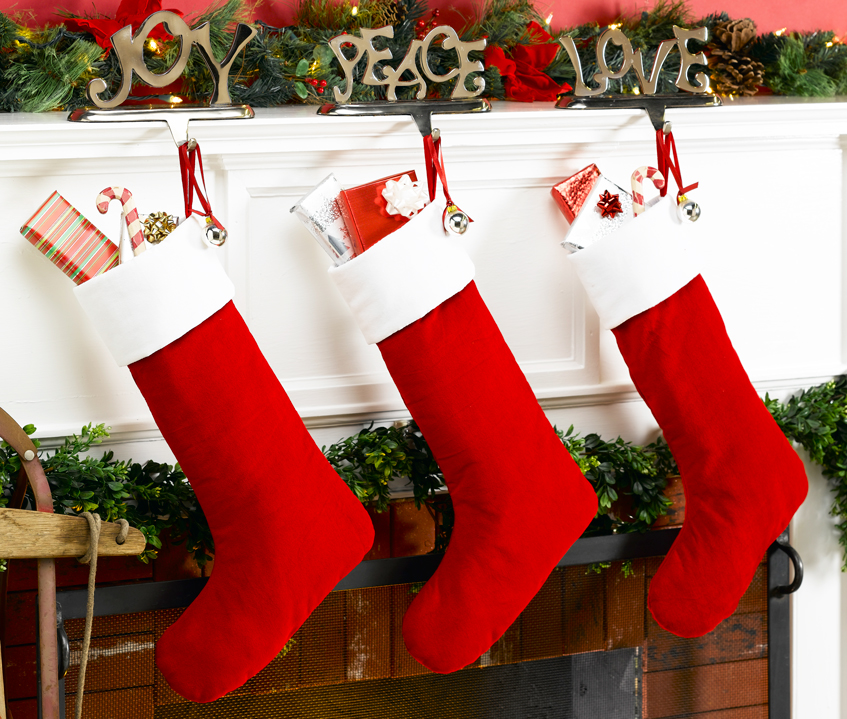
\includegraphics[scale=.2]{stockings.jpg}
      \endmyfig
    \end{center} 
  }
}

\end{document}
% To compile:
%  $ pdflatex *.tex; pdflatex *.tex
